\chapter{Problème du voyageur de commerce}
\label{chap:tsp}

Le problème du voyageur de commerce (TSP) consiste à trouver le plus court chemin passant par chaque ville une et une seule fois, et revenant à la ville de départ. Nous allons employer deux méthodes pour résoudre ce problème : une résolution linéaire avec CPLEX \cite{wiki_tsp} et une résolution par énumération des permutations possibles.

\section{Modélisation}
\label{sec:tsp_model}
On considère un graphe non orienté $G=<S,A>$ où $S$ est l'ensemble des sommets et $A$ l'ensemble des arêtes. À chaque arête $a_{ij}$ est associée une distance $c_{ij}$. On détermine le plus court chemin passant une fois par chaque sommet, et revenant au sommet de départ.

\subsection{Variables}

\begin{itemize}
    \item $x_{ij}$ : vaut 1 si l'arête $a_{ij}$ est empruntée, 0 sinon
\end{itemize}

\subsection{Fonction objectif}

On cherche à minimiser la somme des distances des arêtes empruntées :

\begin{equation}
    \min \sum_{(i,j) \in A} c_{ij} \cdot x_{ij}
\end{equation}

\subsection{Contraintes}

\begin{itemize}
    \item Chaque sommet doit être relié à une arête entrante :
    
    \begin{equation}
        \sum_{i \in S} x_{ik} = 1 \quad \forall k \in S
    \end{equation}
        

    \item Chaque sommet doit être relié à une arête sortante :
    
    \begin{equation}
        \sum_{j \in S} x_{kj} = 1 \quad \forall k \in S
    \end{equation}

    \item Empêcher les sous-cycles :
    
    \begin{equation}
        \sum_{(i,j) \in A} x_{ij} + \sum_{(j,i) \in A} x_{ji} \leq 1 \quad \forall i,j \in S
    \end{equation}
\end{itemize}

Le code Python équivalent à ce modèle est donné en annexe \ref{app:tsp_model}.

\section{Résolution par énumération}

On peut résoudre le problème du TSP en énumérant toutes les permutations possibles des villes, et en calculant la distance totale pour chaque permutation. La solution optimale est celle qui minimise la distance totale.

\begin{algorithm}[H]
    \caption{tsp\_brute\_force}\label{alg:tsp_enum}
    \KwData{$graph$}
    \KwResult{$best\_route$: liste des villes dans l'ordre optimal}

    $min\_cost \gets \infty$\;
    $best\_route \gets []$\;

    \For{$start\_end\_node$ in $graph.nodes$}{
        $remaining\_nodes \gets graph.nodes - start\_end\_node$\;
        \For{$permutation$ in $permutations(remaining\_nodes)$}{
            $route \gets [start\_end\_node] + permutation + [start\_end\_node]$\;
            $cost \gets 0$\;
            \For{$i \gets 0$ \KwTo $len(route)-1$}{
                $cost \gets cost + graph.costs[route[i]][route[i+1]]$\;
            }
            \If{$cost < min\_cost$}{
                $min\_cost \gets cost$\;
                $best\_route \gets route$\;
            }
        }
    }
    \Return $best\_route$\;

\end{algorithm}

\section{Génération de graphes aléatoires}

Nous pouvons implémenter une fonction pour générer des graphes aléatoires de $n$ villes avec des coûts aléatoires. Nous pourrons ainsi tester nos algorithmes sur des graphes de différentes tailles.
Nous choisissons des coûts entre 10 et 50, et les villes ont une probabilité $p$ d'être connectées.

\begin{verbatim}
def gen_tsp(n: int, p: float, file_name: str = "tsp.txt"):
    nodes = [], cost = {}

    for i in range(n):
        nodes.append(i)

    for i in range(n):
        for j in range(i+1, n):
            if random.random() < p:
                cost[(i, j)] = random.randint(10, 50)
                       
    Path("examples").mkdir(parents=True, exist_ok=True)
    with open(f"examples/{file_name}", "w") as f:
        f.write(f"{n} {len(cost)}\n")
        for (i, j), c in cost.items():
            f.write(f"{i} {j} {c}\n")
\end{verbatim}

\section{Résultats et comparaison des méthodes}

Nous pouvons tester nos algorithmes avec un exemple simple fourni par l'énoncé. Ils nous donnent le même résultat :

\begin{figure}[H]
    \centering
    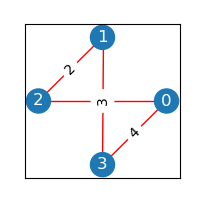
\includegraphics[width=0.5\textwidth]{resources/resol_tsp.png}
    \caption{Résolution d'un exemple simple de TSP}
    \label{fig:resol_bruteforce}
\end{figure}

Nous pouvons désormais comparer le temps d'exécution des deux méthodes en fonction de la taille du graphe. Nous testons les méthodes sur des graphes dont les villes ont une probabilité de connexion de 0.8. Changer cette probabilité ne semble pas avoir un impact significatif sur les résultats.

\begin{table}[H]
    \centering
    \begin{tabular}{|c|c|c|c|c|c|c|}
        \hline
        \textbf{Méthode / Taille du graphe} & 6 & 8 & 10 & 12 & 20 & 30 \\
        \hline
        \textbf{CPLEX} & 0.012 & 0.012 & 0.013 & 0.014 & 0.023 & 0.04 \\
        \hline
        \textbf{Énumération} & 0.00005 & 0.025 & 2.11 & 338.57 & $10^3$ & >> $10^3$ \\
        \hline
    \end{tabular}
    \caption{Temps d'exécution (s) des deux méthodes en fonction de la taille du graphe}
\end{table}

Nous extrapolons les résultats par une régression linéaire pour obtenir une estimation du temps d'exécution pour des graphes de taille supérieure à 12 avec la méthode par énumération.

Nous constatons que la méthode par énumération devient rapidement impraticable pour des graphes de taille supérieure à 10, alors que la méthode CPLEX reste efficace pour des graphes de taille plus importante. Cela est dû à la complexité exponentielle de la méthode par énumération.

\newpage

Voici un autre exemple de résolution du TSP avec un graphe de 20 villes généré aléatoirement : 

\begin{figure}[H]
    \centering
    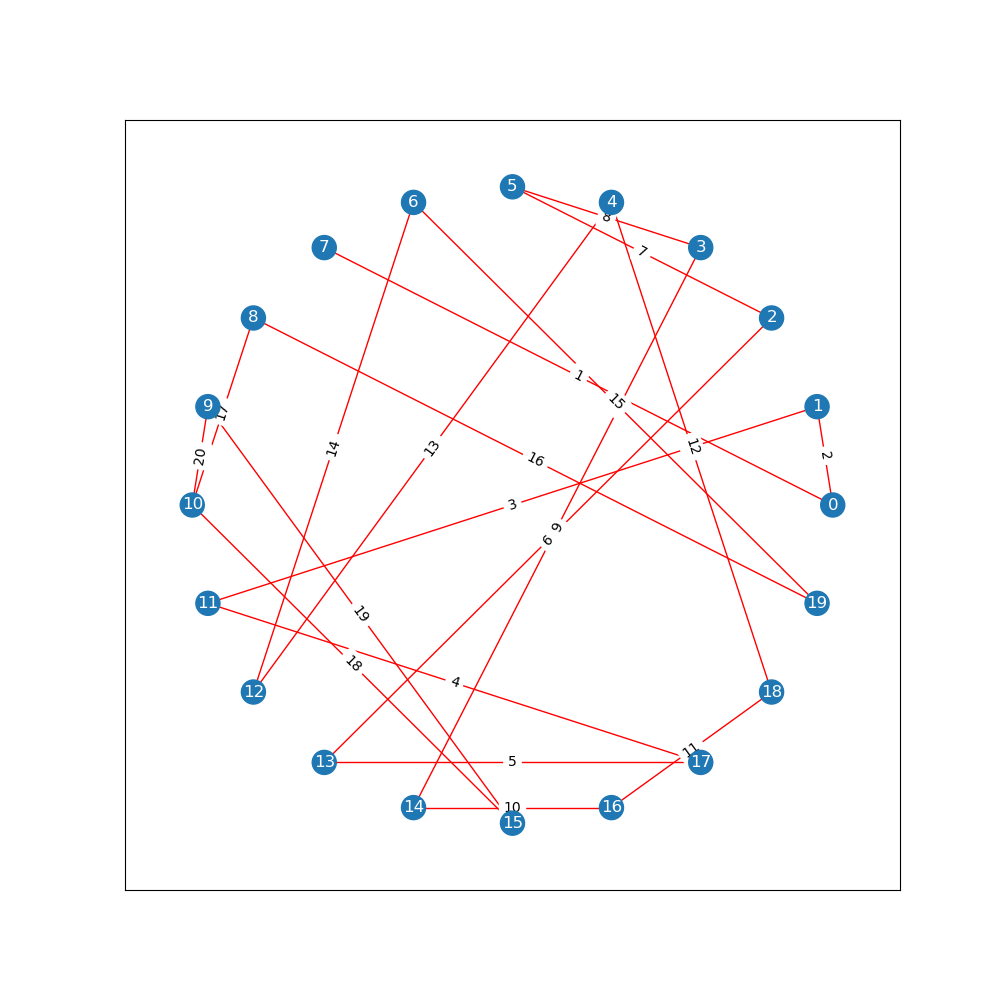
\includegraphics[width=1\textwidth]{resources/20_20_tsp.png}
    \caption{Résolution d'un exemple de TSP avec 20 villes}
    \label{fig:2020_tsp}
\end{figure}